\documentclass[border=4pt]{standalone}
\usepackage{amsmath,amssymb,tikz}
\usetikzlibrary{arrows.meta,calc,matrix,positioning}
\definecolor{figB}{RGB}{31,90,166}\definecolor{figR}{RGB}{176,48,48}\definecolor{figG}{RGB}{46,125,50}\definecolor{figO}{RGB}{214,120,20}
\begin{document}
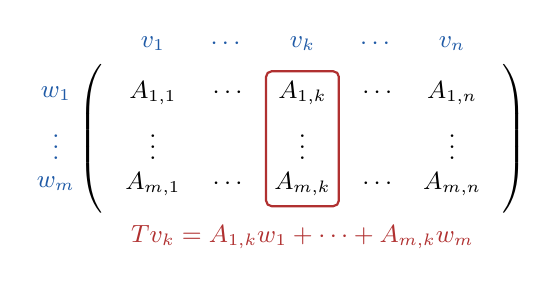
\begin{tikzpicture}
\matrix (M) [matrix of math nodes,left delimiter=(,right delimiter=),
  nodes={minimum width=0.95cm,minimum height=0.55cm,inner sep=1pt,font=\small},
  column sep=0pt,row sep=0pt]
{ A_{1,1} & \cdots & A_{1,k} & \cdots & A_{1,n}\\
  \vdots  &        & \vdots  &        & \vdots \\
  A_{m,1} & \cdots & A_{m,k} & \cdots & A_{m,n}\\};
\draw[figR,thick,rounded corners=2pt] ($(M-1-3.north west)+(0.02,0)$) rectangle ($(M-3-3.south east)+(-0.02,0)$);
\foreach \c/\l in {1/v_1,3/v_k,5/v_n} \node[font=\small,figB] at ($(M-1-\c.north)+(0,0.35)$) {$\l$};
\foreach \c in {2,4} \node[font=\small,figB] at ($(M-1-\c.north)+(0,0.35)$) {$\cdots$};
\foreach \r/\l in {1/w_1,3/w_m} \node[font=\small,figB] at ($(M-\r-1.west)+(-0.75,0)$) {$\l$};
\node[font=\small,figB] at ($(M-2-1.west)+(-0.75,0)$) {$\vdots$};
\node[font=\small,figR,anchor=north] at ($(M-3-3.south)+(0,-0.12)$) {$Tv_k=A_{1,k}w_1+\dots+A_{m,k}w_m$};
\end{tikzpicture}
\end{document}
